\documentclass{article}
\usepackage{marvosym}

%...TikZ & PGF
\usepackage{pgfplots}
\pgfplotsset{compat=1.11}
\tikzset{>=latex}
\usetikzlibrary{calc,math}
\usepackage{tikzsymbols}
\usepgfplotslibrary{fillbetween}
\usetikzlibrary{decorations.markings} 
\usetikzlibrary{arrows.meta} %...APP2 for arrows as objects and images
\usetikzlibrary{backgrounds} %...For shading portions of graphs
\usetikzlibrary{patterns} %...Unit 5 Problems
\usetikzlibrary{shapes.geometric} %...For drawing cylinders in Unit 2
\usepackage{makecell} %...use \thead{} to enable line skip in table headers
\tikzset{
    mark position/.style args={#1(#2)}{
        postaction={
            decorate,
            decoration={
                markings,
                mark=at position #1 with \coordinate (#2);
            }
        }
    }
} %...See https://tex.stackexchange.com/questions/43960/define-node-at-relative-coordinates-of-draw-plot

\tikzset{
    declare function = {trajectoryequation10(\x,\vi,\thetai)= tan(\thetai)*\x - 10*\x^2/(2*(\vi*cos(\thetai))^2);},
    declare function = {trajectoryequation(\x,\vi,\thetai)= tan(\thetai)*\x - 9.8*\x^2/(2*(\vi*cos(\thetai))^2);},
    declare function = {patheq(\x,\yi,\vi,\thetai)= \yi + tan(\thetai)*\x - 9.8*\x^2/(2*(\vi*cos(\thetai))^2);},
    declare function = {patheqten(\x,\yi,\vi,\thetai)= \yi + tan(\thetai)*\x - 10*\x^2/(2*(\vi*cos(\thetai))^2);} %like patheq but with gravity = 10
}

%...siunitx
\usepackage{siunitx}
\DeclareSIUnit{\nothing}{\relax}
\def\mymu{\SI{}{\micro\nothing} }
\DeclareSIUnit\mmHg{mmHg}
\DeclareSIUnit{\mile}{mi}
%...NOTE: "The product symbol between the number and unit is set using the quantity-product option."

%...Other
\usepackage{amsthm}
\usepackage{amsmath}
\usepackage{amssymb}
\usepackage{cancel}
\usepackage{subcaption}
\usepackage{dashrule}
\usepackage{enumitem}
\usepackage{fontawesome}
\usepackage{multicol}
\usepackage{glossaries}
%\numberwithin{equation}{section}
\numberwithin{figure}{section}
\usepackage{float}
\usepackage{twemojis} %...twitter emojis
\usepackage{utfsym}
\usepackage{linearb} %...For \BPwheel in Unit 8
\newcommand{\R}{\mathbb{R}} %...real number symbol
\usepackage{graphicx}
\graphicspath{ {../Figures/} }
\usepackage{hyperref}
\hypersetup{colorlinks=true,
    linkcolor=blue,
    filecolor=magenta,
    urlcolor=cyan,}
\urlstyle{same}
\newcommand{\hdashline}{{\hdashrule{\textwidth}{0.5pt}{0.8mm}}}
\newcommand{\hgraydashline}{{\color{lightgray} \hdashrule{0.99\textwidth}{1pt}{0.8mm}}}

%...Miscellaneous user-defined symbols
\newcommand{\fnet}{F_{\text{net}}} %...For net force
\newcommand{\bvec}[1]{\vec{\mathbf{#1}}} %...bold vector
\newcommand{\bhat}[1]{\,\hat{\mathbf{#1}}} %...bold hat vector
\newcommand{\que}{\mathord{?}}  %...Question mark symbol in equation env
%...Define thick horizontal rule for examples:
\newcommand{\hhrule}{\hrule\hrule}
\let\oldtexttt\texttt% Store \texttt
\renewcommand{\texttt}[2][black]{\textcolor{#1}{\ttfamily #2}}% 

%...For use in the exam document class
\newif\ifprintmetasolutions


%...Decreases space above and below align and gather enironment
\makeatletter
\g@addto@macro\normalsize{%
  \setlength\abovedisplayskip{-3pt}
  \setlength\belowdisplayskip{6pt} 
}
\makeatother







\begin{document}
\begin{center}
    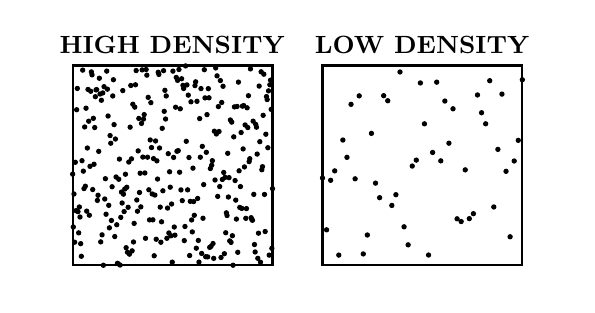
\begin{tikzpicture}[
        declare function={a(\x)=0*\x+2;},
        declare function={b(\x)=0*\x;}
    ]
    \begin{axis}[
        domain=0:5,
        axis lines=middle,
        axis equal image,
        xtick=\empty, ytick=\empty,
        axis line style={draw=none},
        enlargelimits=true,
        clip mode=individual, clip=false
    ]
    \addplot [black, only marks, mark=*, samples=300, mark size=0.75,domain=0:2]
        {0.5*(a(x)+b(x)) + 0.5*rand*(a(x)-b(x))};
        
    \addplot [black, only marks, mark=*, samples=50, mark size=0.75,domain=2.5:4.5]
        {0.5*(a(x)+b(x)) + 0.5*rand*(a(x)-b(x))};
    \draw[thick] (axis cs: 0,0) rectangle (axis cs: 2,2);
    \draw[thick] (axis cs: 2.5,0) rectangle (axis cs: 4.5,2);
    \node at (axis cs: 1,2.2) {\small \textbf{HIGH DENSITY}};
    \node at (axis cs: 3.5,2.2) {\small \textbf{LOW DENSITY}};
    \end{axis}
    \end{tikzpicture}
    \captionsetup{type=figure,margin=1in,font=scriptsize}
    \captionof{figure}{Particles in two boxes of identical size. The air density is higher in the box with more particles.}
\end{center}

\begin{center}
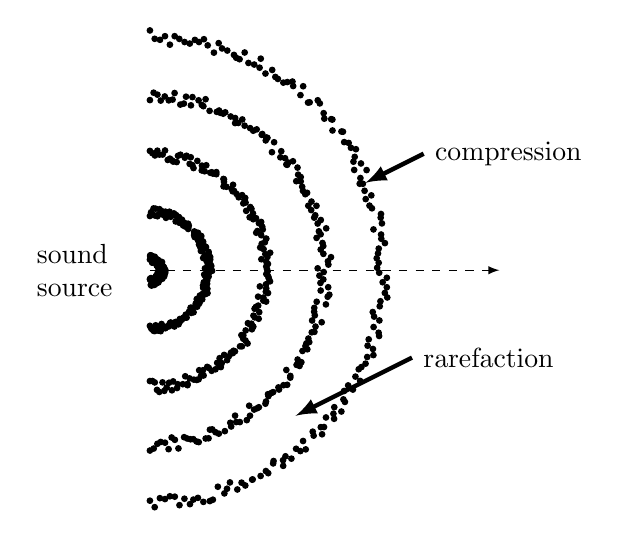
\begin{tikzpicture}
    \begin{axis}[height=7.5cm,width=7.5cm,
      cycle list={
        only marks,mark size=1pt\\
        only marks,mark size=1pt\\
      },
      xmin=0,xmax=8,
      ymin=-4,ymax=4,
      domain=270:360+90,
      samples=150,
      axis line style={draw=none},
      ticks=none,
      clip=false,
    ]
    \draw[dashed,->] (0,0) -- (6,0);
    \addplot ({(0.2+0.07*rand)*cos(x)},{(0.2+0.07*rand)*sin(x)});
    \addplot ({(1.0+0.07*rand)*cos(x)},{(1.0+0.07*rand)*sin(x)});
    \addplot ({(2.0+0.10*rand)*cos(x)},{(2.0+0.10*rand)*sin(x)});
    \addplot ({(3.0+0.12*rand)*cos(x)},{(3.0+0.12*rand)*sin(x)});
    \addplot ({(4.0+0.12*rand)*cos(x)},{(4.0+0.12*rand)*sin(x)});
    
    \draw[<-,ultra thick] (3.7,1.5) -- ++(axis direction cs: 1,0.5) node[right] {compression};
    \draw[<-,ultra thick] (2.5,-2.5) -- ++(axis direction cs: 2,1) node[right] {rarefaction};
    
    \node[align=left,left=1em] at (0,0) {sound\\ source};
    \end{axis}
\end{tikzpicture}
\end{center}

\end{document}